%--------------------------------------------------------------------
% Эта преамбула с комментариями для написания лабораторных работ по
% физике. В его основе информация из книги С. М. Львовского "Набор и
% верстка в пакете Latex", а также материалы по курсу "Документы и
% презентации в Latex" от ВШЭ https://www.coursera.org/learn/latex. Ну
% и мой опыт (1 год и 16 лабораторных работ)
% Автор - Баринов Леонид
% Дата - 06.08.2019
%--------------------------------------------------------------------
%--------------------------------------------------------------------
% Для начала необходимо определиться с типом документа. Оптимальный
% (на мой взгляд) вариант - article. Также существуют типы book,
% report, proc и другие. Также в необязательном аргументе можно
% указать тип страницы и размер шрифта. Стандарт по умолчанию - А4 и
% 12 (иногда 10) шрифт. Необязательный аргумент шрифта может принимать
% только 3 параметра - 10, 11, 12 (pt).

\documentclass[a4paper, 12pt]{article}

%--------------------------------------------------------------------
% Чтобы использовать другие размеры шрифта используется пакет
% extsizes. Он позволяет указывать в \documentclass такие размеры - 8,
% 9, 10, 11, 12, 14, 17, 20 (pt). При указании других размеров могут
% возникать различные проблемы.

\usepackage{extsizes}

%--------------------------------------------------------------------
% Необходимо определиться с кодировкой документа. Идеального варианта
% для русского языка не существует - каждый чем-то немного плох. Для
% особо интересующихся - Приложение И в 5 издании книги Львовского. Я
% воспользовался вариантом, предлагаемым на курсе по Latex от ВШЭ.

\usepackage[T2A]{fontenc}
\usepackage[utf8]{inputenc}

%--------------------------------------------------------------------
% Для соблюдения типографских традиций (оказывается такие существуют)
% различных стран создан пакет babel. Самое заметное его действие -
% latex научиться переносить слова того языка, который вы укажите.
% Можно указать несколько языков через запятую. Основной язык
% документа указывается последним.

\usepackage[english,russian]{babel}

%--------------------------------------------------------------------
% Перейдем к заданию полей документа. Есть несколько способов, но
% самый простой из них - это воспользоваться пакетом geometry, который
% позволяет определить все поля документа (начиная с краев листа, что
% важно, так как некоторые другие способы позволяют это сделать только
% косвенно)

\usepackage{geometry}
\geometry{top=25mm}
\geometry{bottom=35mm}
\geometry{left=35mm}
\geometry{right=20mm}

%--------------------------------------------------------------------
% От полей логично перейти к колонтитулам. Тут нам поможет пакет
% fancyhdr. Для него существует 6 колонтитулов - верхний, левый;
% верхний, по центру; верхний, правый и такие же нижние. По умолчанию
% номер страницы находится снизу по центру, а также существует
% линейка, очерчивающие верхний колонтитул. Мне показалось интересным
% сделать колонтитулы схожие с колонтитулами в лабнике. 

\usepackage{fancyhdr}
\pagestyle{fancy}
\renewcommand{\sectionmark}[1]{\markboth{#1}{}} 
% \renewcommand{\headrulewidth}{0mm} % Если необходимо убрать линейку,
% или изменить ее длину
% \lfoot{} % Нижний левый
% \rfoot{} % Нижний правый
% \rhead{} % Верхний правый
% \chead{} % Верхний в центре
\lhead{\thepage} % Номер страницы в левом верхнем углу
\cfoot{} % Оставить нижний колонтитул без цифры

%--------------------------------------------------------------------
% Самое время научиться работать с формулами. А точнее добавить пакеты
% от Американского математического общества, которые позволять
% пользоваться большим количеством математических символов.

\usepackage{amsmath,amsfonts,amssymb,amsthm,mathtools}

%--------------------------------------------------------------------
% Также очень хочется пользоваться русскими буквами в формулах, для
% этого подключаем пакет mathtext, который добавляет окружение
% \text{}. Внутри него можно писать русские буквы в математическом
% режиме.

\usepackage{mathtext}

%--------------------------------------------------------------------
% Большим преимуществом вашего pdf документа будет возможность поиска
% в нем по словам или буквами. (Например, в Ивановнике это
% невозможно)

\usepackage{cmap}

%--------------------------------------------------------------------
% Куда же в физике без картинок и графиков? Давайте исправим
% эту недоработку

\usepackage{graphicx}
\graphicspath{images/} % Необходимо, если рисунки
% находятся в другой папке

%--------------------------------------------------------------------
% graphicx не позволяет вставлять обтекаемые рисунки, но на
% практике они очень нужны. Для этого существует пакет wrapfig

\usepackage{wrapfig}

%--------------------------------------------------------------------
% latex вставляет рисунки по определенному алгоритму. Его,
% конечно, можно менять, но это не настолько просто. Как
% правило, хочется, чтобы картинка располагалась там, где мы это
% указали в коде. Для этого существует несколько пакетов, один из
% них floatrow. Он позволяет для окружения figure указывать
% необязательный аргумент - H (именно большое h), что на latex'овском
% языке означает: вставить картинку здесь и только здесь. (даже если
% облик документа несколько пострадает)

\usepackage{floatrow}

%--------------------------------------------------------------------
% По правилам оформления рисунок всегда должен быть подписан. Для
% этого существует команда \caption{}. Но обычные настройки caption
% меня не совсем устроили. Хотелось сделать подпись меньше
% основного шрифта, а также слово Рис жирным и использовать
% разделитель точку, а не двоеточие. В этом помогает пакет,
% который называется caption (совпадение?)

\usepackage[margin=10pt,font=small,labelfont=bf,labelsep=period]{caption}

%--------------------------------------------------------------------
% Последним важным пунктом остались таблицы. Ведь куда-то нужно
% заносить результаты измерений. На данный момент во время выполнения
% лабораторных работ я заношу результаты в таблицу excel, а потом с
% помощью сайта www.tablesgenerator.com превращаю в таблицу latex и
% дооформляю.

\usepackage{array,tabularx,tabulary,booktabs}

%--------------------------------------------------------------------
% После excel есть ощущения, что везде объединить колонки или строки
% легко. В latex не совсем так. Помогают пакеты multirow, multicol. 

\usepackage{multirow}
\usepackage{multicol}

%--------------------------------------------------------------------
% Иногда могут потребоваться длинные таблицы на несколько страниц.
% Обычные таблицы latex воспринимает как одну букву. И
% становиться понятно, почему возникают проблемы при переносе
% обычной таблицы. (Ведь нельзя же перенести одну букву!). Поэтому
% вместо обычной таблицы нужна длинная таблица.

\usepackage{longtable}

%--------------------------------------------------------------------
% Часто в таблице хочется сделать перенос текста или формулы. Просто
% так это сделать не получиться из-за синтаксиса tabular. Для этого
% каждый раз необходимо создавать новое окружение tabular, что
% утомительно. Поэтому можно ввести команду \specialcell
% (назвать можно по-любому)
    
\newcommand{\specialcell}[2][c]{%
	\begin{tabular}[#1]{@{}c{}}#2\end{tabular}}

%--------------------------------------------------------------------
% Когда в таблице много колонок и строк, кажется, что они находятся
% слишком близко к друг другу. Можно переопределить
% несколько параметров, чтобы выглядело лучше. Это можно сделать либо
% в преамбуле, либо непосредственно в документе. Первое
% переопределение отвечает за интервал между строками, второе за
% интервал между колонками

% \renewcommand{\arraystretch}{1.8} 
% \renewcommand{\tabcolsep}{1cm} 

%--------------------------------------------------------------------
% В русской типографской традиции принято начинать каждый новый абзац
% с красной строки. Даже первый после заголовка (или подзаголовка).
% Чтобы каждый раз не ставить красную строку вручную существует пакет
% indentfirst

\usepackage{indentfirst}

%--------------------------------------------------------------------
% Некоторые модификаторы начертания

\usepackage{soul}
\usepackage{soulutf8}
 
\usepackage{mathrsfs}
\usepackage[e]{esvect}
\newcommand{\dive}{\mathrm{div}}
\newcommand{\rot}{\mathrm{rot}}
\begin{document}
\renewcommand{\vv}{\vec}
\thispagestyle{empty}
\begin{center}
    \textit{Федеральное государственное автономное образовательное\\ учреждение высшего образования }

    \vspace{0.5ex}

        \textbf{«Московский физико-технический институт\\ (национальный исследовательский университет)»}
\end{center}

\vspace{10ex}

\begin{center}
    \vspace{13ex}

    \so{\textbf{Лабораторная работа №-.-.-}}

    \vspace{1ex}

    по курсу общей физики

    на тему:

    \textbf{\textit{<<>>}}

    \vspace{30ex}

    \begin{flushright}
        \noindent
        \textit{Работу выполнил:}\\  
        \textit{Баринов Леонид \\(группа Б02-827)}
    \end{flushright}
    \vfill
    Долгопрудный \\2019
\newpage
\setcounter{page}{1}
\fancyhead[R]{\nouppercase{\leftmark}}	
\end{center}

\section{Аннотация}
В работе будут рассмотрены принципы работы
униполярных машин, их преимущества и
недостатки, а также приведены примеры их
использования в промышленности.

На примере простейшей униполярной
машины, вращающегося вокруг своей оси
симметрии магнитного диска, будет
проведена проверка закона
электромагнитной индукции Фарадея.

\section {Теоретические сведения}
\subsection{Электромагнитная индукция}

Открытие электромагнитной индукции
Фарадеем в 1831 г. было одним из
наиболее фундаментальных открытий в
электродинамике Для демонстрации этого
явления возьмем неподвижный магнит и
проволочную катушку, концы которой
соединим с гальванометром. Если катушку
приближать к одному из полюсов магнита,
то во время движения стрелка
гальванометра отклоняется — в катушке
возбуждается электрический ток. При
движении катушки в обратном направлении
направление тока меняется на
противоположное. То же самое происходит,
если повернуть магнит на 180$^\circ$, не меняя
направления движения катушки. Магнит
можно заменить другой катушкой с током
или электромагнитом. Вообще, при
движении катушки в постоянном магнитном
поле в ней (за исключением некоторых
специальных случаев, которые выяснятся
ниже) возбуждается электрический ток,
прекращающийся, когда катушка
останавливается. Этот ток называется
индукционным током, а самое явление —
электромагнитной индукцией. В
частности, когда катушка равномерно
вращается в постоянном магнитном поле,
индукционный ток периодически меняет
свою силу и направление.

Возбуждение электрического тока при
движении проводника в магнитном поле
объясняется действием силы Лоренца,
возникающей при движении проводника.
Рассмотрим сначала простейший случай,
когда два параллельных провода $AB$ и
$CD$  
помещены в постоянное однородное
магнитное поле, перпендикулярное к
плоскости рисунка и направленное к
читателю (рис. 1). Слева провода $AB$ и
$CD$ замкнуты, справа — разомкнуты. 

\begin{wrapfigure}{r}{0.4\linewidth}
    \includegraphics[width=\linewidth]{1}
    \captionsetup{justification=centering}
    \caption{}
\end{wrapfigure}
Вдоль проводов может свободно скользить
проводящий мостик $BC$ . Когда мостик
движется вправо со скоростью $v$ , вместе с
ним движутся электроны и положительные
ионы. На каждый движущийся заряд $e$ в
магнитном поле действует сила Лоренца
$\vv{F} = (e/c)[\vv{v}, \vv{B}]$. На
положительный ион она действует вниз, на
отрицательный электрон — вверх. В
результате электроны начнут перемещаться
по мостику вверх, т. е. по нему потечет
электрический ток, направленный вниз.
Это и есть индукционный ток.
Перераспределившиеся заряды создадут
электрическое поле, которое возбудит
токи и в остальных участках контура
$ABCD$ . На рис. 1 эти токи изображены
сплошными стрелками.

Сила Лоренца $F$ в описанном опыте играет
роль сторонней силы, возбуждающей
электрический ток. Соответствующая
напряженность стороннего поля равна
\[ \vv{E}^{\text{стор}} =
\cfrac{\vv{F}}{e} =
\cfrac{1}{c}[\vv{v}, \vv{B}] \]
Электродвижущая сила, создаваемая этим
полем, называется электродвижущей силой
индукции и обозначается
$\mathscr{E}^\text{инд}$. В
рассматриваемом случае
$\mathscr{E}^\text{инд} = -(v/c)Bl$, где
$l$ -- длина мостика. Знак минус
поставлен потому, что стороннее поле
$(1/c)[\vv{v},\vv{B}] $ направлено
против положительного обхода контура,
определяемого вектором $\vv{B}$ по
правило правого винта. На рис. 1
приращение площади контура $ABCD$ в
единицу времени, или скорость скорости
приращения этой площади. Поэтому
величина 
$v B l$ равна $d\Phi/dt$, т.е. скорости
приращения магнитного потока,
пронизывающего площадь контура $ABCD$.
Таким образом, 

\begin{equation}
    \mathscr{E}^\text{инд} = -
    \frac{1}{c} \frac{d\Phi}{dt}
    \label{eq:base}
\end{equation}

Результат \eqref{eq:base} справедлив и в том
случае, когда однородное магнитное поле
В направлено под любым углом к плоскости
контура $ABCD$ . Действительно, представим
вектор $\vv{B}$ в виде
$\vv{B}_t+\vv{B}_n$ , где $\vv{B}_t$ ---  
тангенциальная, а $\vv{B}_n$  — нормальная к
плоскости контура слагающие этого
вектора. Вектор $\vv{B}_t$  вносит в стороннее
поле слагаемое $(1/c)[\vv{v}, \vv{B}_t]$,
перпендикулярное к мостику. Оно вызывает
лишь перераспределение электрических
зарядов поперек мостика, но тока не 
дает. Ток вызывается только нормальной
слагающей $\vv{B}_n$ , а потому инд определяется
прежней формулой \eqref{eq:base}.

Теперь не составляет труда
распространить формулу \eqref{eq:base} на случай
любого замкнутого провода, движущегося
произвольным образом в постоянном
неоднородном магнитном поле. Для этого
надо мысленно разбить провод на
бесконечно малые участки и рассмотреть
движение каждого из них. При бесконечно
малом перемещении каждого из таких
участков магнитное поле, в котором он
движется, можно считать однородным.
Поэтому электродвижущая сила,
действующая между концами участка, может
быть представлена выражением
\eqref{eq:base}.
Путем суммирования таких выражений
получится формула того же вида,
в которой, однако, под
$\mathscr{E}^\text{инд}$ следует
понимать полную электродвижущую силу,
действующую в замкнутом проводе, а под
$d\Phi/dt$ --- скорость изменения магнитного
потока через любую поверхность,
натянутую на контур провода.

Формула \eqref{eq:base} выражает основной закон
электромагнитной индукции. Она
показывает, что при движении замкнутого
провода в магнитном поле в нем
возбуждается электродвижущая сила,
пропорциональная скорости приращения
магнитного потока, пронизывающего контур
провода.

К формуле \eqref{eq:base} можно прийти также с
помощью закона сохранения энергии, как
это впервые сделал Гельмгольц.

Рассмотрим, следуя Гельмгольцу,
замкнутый виток провода, в который
включен гальванический элемент с
электродвижущей силой Виток движется в
постоянном магнитном поле (вообще
говоря, неоднородном). За время dt
амперовы силы совершают над витком
работу $(I/c)d\Phi$. Кроме того, в витке
выделяется джоулево тепло $RI^2dt$ . Сумма
этих величин должна равняться работе
гальванического элемента $\mathscr{E} I
dt$, т.е.

\begin{equation}
    \frac{1}{c}Id\Phi + I^2Rdt =
    \mathscr{E}I dt
\end{equation}
Отсюда
\begin{equation}
    I =
    \frac{\mathscr{E}-(1/c)d\Phi/dt}{R}
    \label{eq:helm}
\end{equation}

Таким образом, в движущемся витке ток
определяется не только электродвижущей
силой гальванического элемента. К ней
добавляется слагаемое $-(1/c)d\Phi/dt$ . Это
слагаемое и есть электродвижущая сила
индукции.

Заметим, что уравнению сохранения
энергии \eqref{eq:base} можно также
удовлетворить, положив $I=0$ . Какое из
двух решений выбрать: решение $I=0$  или
решение \eqref{eq:helm} --- на это закон сохранения
энергии не дает никаких указаний.
Следовательно, без привлечения
дополнительных соображений он не
позволяет предсказать явление
электромагнитной индукции. Нужно как-то
исключить решение $I = 0$. С этой целью,
как это сделал Гельмгольц, в виток и
включен гальванический элемент с
электродвижущей силой $\mathscr{E}$ . То
обстоятельство, что добавочная
электродвижущая сила $-(1/c)d\Phi/dt$,
появляющаяся при движении проводника, не
зависит от $\mathscr{E}$, делает правдоподобным
заключение, что и при отсутствии
гальванического элемента в движущемся
витке должна возникнуть такая же
электродвижущая сила. Можно обойтись и
без введения гальванического элемента,
если предположить, что при движении
проводника должен возникать индукционный
ток. Тогда закон сохранения энергии
позволяет определить силу этого тока, а
следовательно, и электродвижущую силу
индукции. В этом истинный смысл и
содержание рассуждения Гельмгольца.

Индукционные токи могут
возникать и в неподвижных проводниках.
Действительно, возьмем замкнутый провод
и постоянный магнит. При движении
провода возникает индукционный ток. Что
произойдет, если, оставляя провод
неподвижным, двигать магнит? Покой и
движение — понятия относительные.
Явление индукционного тока должно
зависеть только от относительного
движения провода и магнита. Отсюда
следует, что при движении магнита будет
возбуждаться такой же индукционный ток,
что и при соответствующем движении
провода. Опыт подтверждает это
заключение. Возьмем прежнюю катушку,
соединенную с гальванометром, и будем
приближать к ней магнит. Стрелка
гальванометра отклонится — в катушке
возбудился электрический ток. При
удалении магнита стрелка отклоняется в
противоположную сторону, т.е.
индукционный ток меняет направление. То
же самое происходит, если магнит
повернуть к катушке другим полюсом, не
меняя направления его движения. Если
магнит вращать, то индукционный ток в
катушке будет периодически менять свое
направление. Когда магнит
останавливается, индукционный ток в
катушке прекращается. Вместо магнита
можно взять электромагнит или другую
катушку, по которой течет ток,
возбуждающий магнитное поле. При их
движении в неподвижной катушке
возбуждается электрический ток.

В описанных опытах с движением магнита
менялся магнитный поток, пронизывающий
неподвижную катушку. Но такое же
изменение магнитного потока можно
получить и без движения магнита.
Достаточно поместить катушку в
переменное магнитное поле. Последнее
можно подобрать так, чтобы в месте
нахождения катушки оно в точности
совпадало с магнитным полем движущегося
магнита. От такой замены объективные
физические условия, в которых находится
катушка, не изменятся. Поэтому
естественно ожидать, что не изменится и
индукционный ток, возбуждаемый в
катушке. Опыт подтверждает и это
заключение. Возьмем две неподвижные
катушки, одна из которых помещена внутри
другой. Если через одну из катушек
пропускать переменный ток, то в другой
катушке появляется индукционный
электрический ток. Таким образом, для
возбуждения индукционного тока
существенно изменение магнитного потока
через контур проводника, а не способ,
каким это изменение достигается.

\begin{wrapfigure}[7]{r}{0.3\linewidth}
    \vspace{-20pt}
    \includegraphics[width=\linewidth]{2}
    \captionsetup{justification=centering}
    \caption{}
\end{wrapfigure}

Вот другая демонстрация, подтверждающая
это заключение. На подковообразный
магнит надевается проволочная катушка,
соединенная с гальванометром (рис.~2).
Если полюсы магнита замкнуть железным якорем, то изменится магнитный
поток через катушку. В ней возникает
индукционный ток, и стрелка
гальванометра отклоняется.

\subsection{Правило Ленца}
Формула \eqref{eq:base} определяет не
только
величину, но и направление индукционного
тока.

\begin{wrapfigure}{l}{0.2\linewidth}
    \includegraphics[width=\linewidth]{3}
    \captionsetup{justification=centering}
    \caption{}
\end{wrapfigure}

\noindent Действительно, возьмем в магнитном
поле замкнутый проволочный виток,
положительное направление обхода
которого составляет с направлением поля
правовинтовую систему (на рис. 3 
магнитное поле направлено к читателю).
Допустим, что магнитный поток $\Phi$  
возрастает. Тогда, согласно формуле
\eqref{eq:base}, величина инд будет
отрицательна, а потому индукционный ток
в витке потечет в отрицательном
направлении. Такой ток, ослабляя внешнее
магнитное поле, будет препятствовать
возрастанию магнитного потока. Пусть
теперь магнитный поток $\Phi$ убывает.
Тогда величина $\mathscr{E}^\text{инд}$
станет положительной, а индукционный ток
в витке потечет в положительном
направлении и будет препятствовать
убыванию магнитного поля и магнитного
потока. Таким образом, индукционный ток
всегда имеет такое направление, что он
ослабляет действие причины, возбуждающей
этот ток.

\subsection{Максвелловская трактовка
явления электромагнитной индукции}
Когда проводник движется в
постоянном магнитном поле, индукционный
ток вызывается магнитной составляющей
силы Лоренца $(e/c)[\vv{v},\vv{B}]$. Какая же сила
возбуждает индукционный ток в
неподвижном проводнике, находящемся в
переменном магнитном поле? Ответ был дан
Максвеллом. Согласно Максвеллу, всякое
переменное магнитное поле возбуждает в
окружающем пространстве электрическое
поле. Последнее и является причиной
возникновения индукционного тока в
проводнике. Максвеллу принадлежит
следующая углубленная формулировка
закона электромагнитной индукции.

Всякое изменение магнитного поля во
времени возбуждает в окружающем
пространстве электрическое поле.
Циркуляция вектора напряженности $\vv{E}$ этого
поля по любому неподвижному замкнутому
контуру $s$ определяется выражением

\begin{equation}
    \oint\limits_s (\vv{E} d\vv{s}) =
    - \frac{1}{c}
    \frac{\partial\Phi}{\partial t},
    \label{eq:maxvel}
\end{equation}
где $\Phi$ --- магнитный поток,
пронизывающий контур $s$. Мы
использовали для обозначения скорости
изменения магнитного потока знак
частной, а не полной производной. Этим
мы хотим подчеркнуть, что контур $s$  
должен быть неподвижным.

Между максвелловым и фарадеевым
пониманием явления электромагнитной
индукции имеется существенное различие.
Согласно Фарадею, электромагнитная
индукция состоит в возбуждении
электрического тока. Для ее наблюдения
необходимо наличие замкнутого
проводника. Максвелл, напротив, видит
сущность электромагнитной индукции
прежде всего в возбуждении
электрического поля, а не тока.
Электромагнитная индукция может
наблюдаться и тогда, когда в
пространстве вообще нет никаких
проводников. Появление индукционного
тока в замкнутом проводнике при внесении
последнего в переменное магнитное поле
есть лишь одно из проявлений
электрического поля $\vv{E}$ , возникшего в
результате изменения поля магнитного. Но
поле $\vv{E}$ может производить и другие
действия, например поляризовать
диэлектрик, вызвать пробой конденсатора,
ускорять и тормозить заряженные частицы
и т.п. Оно может вызвать электрический
ток и в незамкнутом проводнике, как
показывает, например, следующий опыт.

Возьмем две катушки, расположенные
близко одна от другой приблизительно
так, чтобы ось одной катушки была
продолжением оси другой. Концы первой
катушки присоединим к звуковому
генератору, т.е. прибору, который может
возбуждать переменные токи с частотами,
лежащими в звуковом диапазоне. Концы
второй катушки соединим с
горизонтальными пластинами электронного
осциллографа. Когда в первой катушке
течет переменный ток, луч осциллографа
отклоняется, хотя цепь второй катушки
разомкнута. Луч бегает вверх и вниз, и
на экране видна светлая вертикальная
полоска, переходящая в синусоиду после
включения горизонтальной развертки. Это
доказывает, что между горизонтальными
пластинами осциллографа появилось
переменное электрическое поле. Пластины
оказались заряженными, причем их заряды
периодически меняются во времени, а во
второй катушке текут переменные
индукционные токи, несмотря на то, что
цепь разомкнута.

Максвеллова формулировка закона индукции
более общая, чем формулировка Фарадея.
Она принадлежит к числу наиболее важных
обобщений электродинамики. Математически
закон индукции в понимании Максвелла
выражается формулой \eqref{eq:maxvel}, где s —
произвольный математический замкнутый
контур, который может быть проведен и в
диэлектрике, а не обязательно в
проводнике, как было у Фарадея.
Магнитный поток $\Phi$ определяется
интегралом

\begin{equation}
    \Phi = \oint\limits_S \vv{B}d\vv{S}
    \label{eq:potok}
\end{equation}
взятым по произвольной поверхности $S$,
натянутой на контур $s$. Поэтому формулу
\eqref{eq:maxvel} можно представить в
виде

\begin{equation}
    \oint\limits_s(\vv{E}d\vv{s}) = -
    \frac{1}{c} \frac{\partial}{\partial
    t} \int\limits_S \vv{B} d\vv{S} = -
    \frac{1}{c} \int\limits_S
    \frac{\partial \vv{B}}{\partial
    t}d\vv{S}
    \label{eq:eq}
\end{equation}
Уравнение \eqref{eq:eq} может быть
преобразовано в дифференциальную форму
\begin{equation}
    \rot 
    \vv{E} = - \frac{1}{c} \frac{\partial
        \vv{B}}{\partial t}
    \label{eq:rot}
\end{equation}
Это --- дифференциальная форма закона
электромагнитной индукции. 

В электростатике источниками
электрического поля являются неподвижные
электрические заряды. Для такого поля
интеграл $\oint \vv{E}d\vv{s}$ обращается в нуль по
любому замкнутому контуру. По этой
причине одно только электростатическое
поле не может обеспечить непрерывное
течение электричества вдоль замкнутых
проводов. Напротив, электрическое поле,
возбуждаемое магнитным полем, меняющимся
во времени, — не потенциальное, а
вихревое. Ротор такого поля и его
циркуляция, вообще говоря, отличны от
нуля. Благодаря этому вихревое поле без
каких бы то ни было добавочных сил может
вызвать непрерывное течение
электричества по замкнутым проводам. Это
течение и наблюдается в виде
индукционных токов.

\subsection{Нерелятивистское
    преобразование полей $B$ и $H$ 
при переходе от одной инерциальной
системы к другой}

Пусть заряженная частица в системе
отсчета $S$ движется со скоростью
$\vv{v}$ в полях $\vv{E}$ и $\vv{B}$.
Тогда на нее действует сила 

\[
    \vv{F} = q\left(\vv{E} +
    \frac{1}{c}[\vv{v}, \vv{B}] \right)
\]

Перейдем в систему отсчета $S'$,
движущуюся со скоростью $\vv{v}$, в
которой частица покоится. В этом системе
не частицу действует только сила со
стороны электрического поля:

\[
    \vv{F}' = q \vv{E}'
\]

В нерелятивистском пределе сила есть
инвариант, то есть $\vv{F} = \vv{F}'$.
Отсюда следует первый закон
преобразования:

\begin{equation}
    \vv{E}' = \vv{E} + \frac{1}{c}
    [\vv{v}, \vv{B}]
    \label{eq:E}
\end{equation}

Обратный переход от системы отсчета $S'$
к системе $S$ получается изменением
знака скорости:

\begin{equation}
    \vv{E} = \vv{E}' -
    \frac{1}{c}[\vv{v}, \vv{B}'] 
\end{equation}

Из закона Био-Савара следует, что
магнитное поле заряда, движущегося со
скоростью $v$, равно 

\[
    \vv{B} =
    \frac{1}{c}[\vv{v},\vv{E}'], \;
    \vv{E}' = \frac{q\vv{r}}{r^3}
\]

Рассмотрим систему покоящихся (в системе
отсчета $S'$) заряженных частиц. Они
создают электростатическое поле


\[
    \vv{E}' = \sum\limits_k
    \frac{q_k}{r_k^3} \vv{r}_k =
    \sum\limits_k \vv{E}'_k
\]

Перейдем в систему отсчета $S$,
движущуюся со скорости $\vv{v}$. Тогда
каждый из зарядов системы создает
магнитное поле $\vv{B}_k =
\frac{1}{c}[\vv{v}, \vv{E}'_k]$, а все
вместе они создают поле 

\[
    \vv{B} = \frac{1}{c} [\vv{v},
    \vv{E}']
\]

Таким образом , в системе отсчета, в
которой заряды движутся, возникает
магнитное поле. Если в собственной
системе зарядов присутствует магнитное
поле $\vv{B}'$ (создаваемое, например,
собственным магнитным моментом частицы),
то суммарное магнитное поле дается
формулой 
\begin{equation}
    \vv{B} = \vv{B}' + \frac{1}{c}
    [\vv{v}, \vv{E}']
    \label{eq:B}
\end{equation}

Обратный переход от системы $S$ к
системе $S'$ получается изменение знака
скорости:
\begin{equation}
    \vv{B}' = \vv{B} - \frac{1}{c}
    [\vv{v}, \vv{E}]
    \label{eq:B'}
\end{equation}

\subsection{Униполярная машина}
В своем принципе униполярная машина
состоит из вращающегося вокруг своей оси
цилиндрического постоянного магнита.
Если при помощи скользящих контактов $A$
и $B$ присоединиться проводник к оси и к
боковой поверхности вращающегося магнита
(рис. 4)
напряженность электромагнитного поля и
плотность тока в каждой точке
пространства будут постоянными во
времени. 

\begin{wrapfigure}[11]{l}{0.2\linewidth}
    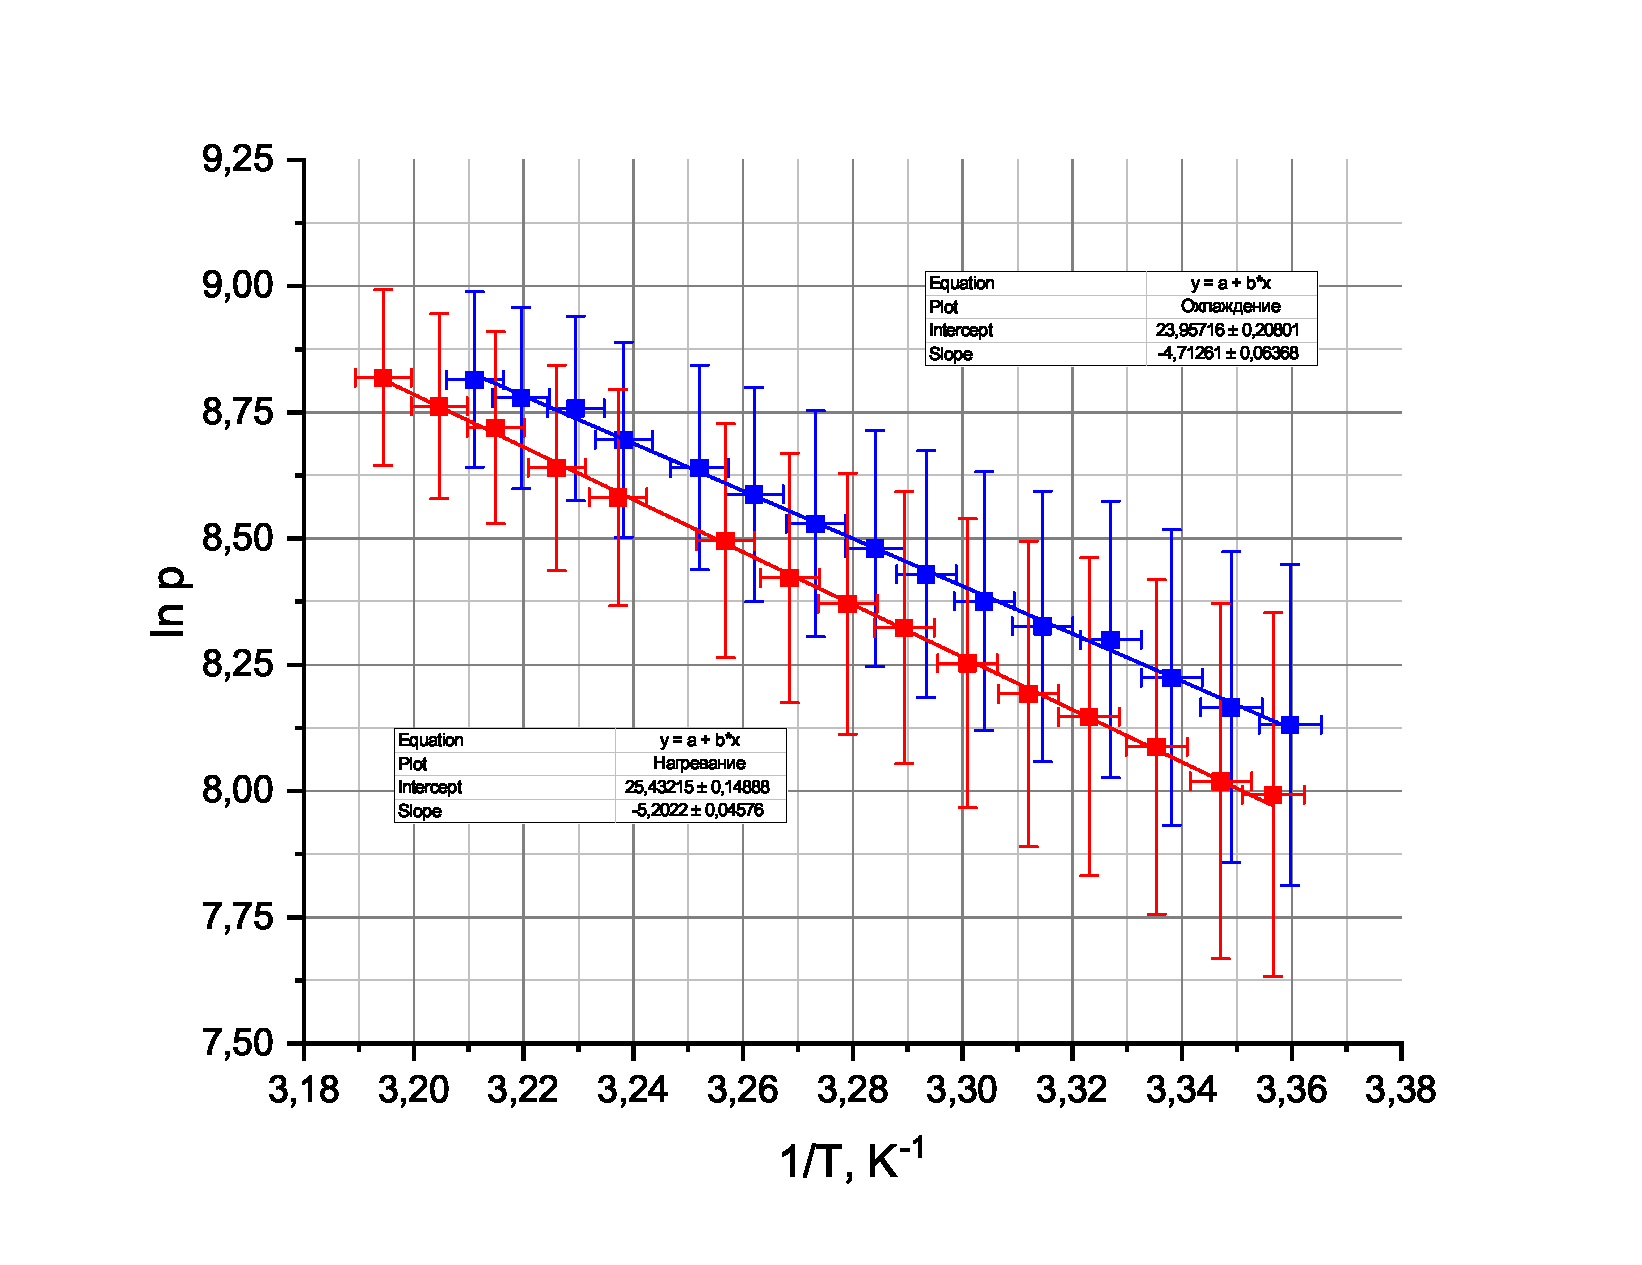
\includegraphics[width=\linewidth]{4}
    \captionsetup{justification=centering}
    \caption{}
\end{wrapfigure}

Применим закон индукции к какому-либо
контуру, проходящему по внешнему проводу
$AVB$ и по магниту, например к контуру
$COAVBC$. В момент времени $t+\Delta t$
материальные точки, находившиеся в
момент $t$ на этом контуре, сместятся на
расстояние $\vv{u}dt$ и займут положение
$C'OAVBC$. Обозначим эти потоки
соответственно через $\Psi$ и $\Psi'$,
так что $d\Psi = \Psi - \Psi'$. Однако
контур $C'OAVBC$ в отличие от контура
$COAVBC$ не замкнут, так что, строго
говоря, понятие потока $\Psi'$ через
этот незамкнутый контур не является
определенным.

Из \eqref{eq:eq} следует, что в
рассмотренном случае под $d\Psi/dt$ надо
понимать величину 

\[
    \frac{d\Psi}{dt} = \oint
    \vv{B}[\vv{u}, d\vv{s}],
\]
причем интеграл должен быть взят по
замкнутому контуру $COAVBC$. Так как
$\vv{u} d\vv{s} \neq 0$ только на
участке $CO$ этого контура, то

\[
    d\Psi = \int\limits_C^O
    \vv{B}[\vv{u}dt, d\vv{s}]
\]

Легко убедится, что это выражение для
$d\Psi$ с точностью до величин второго
порядка относительно $dt$ равно потоку
индукции через бесконечно малый круговой
сектор $COC'$. Поэтому при вычислении
$d\Psi$ из соотношения $d\Psi = \Psi' -
\Psi$ под $\Psi'$ можно понимать поток
через замкнутый контур $C'OAVBCC'$,
получающийся замыканием деформированного
движением контура $C'OAVBC$ отрезком
$CC'$ траектории, описанной точкой $C'$
разрыва контура. 

ЭДС индукции $\mathscr{E}^\text{инд}$ в
контуре $COAVBC$ равна

\[
    \mathscr{E}^\text{инд} =
    -\frac{1}{c} \frac{d\Psi}{dt} = -
    \frac{1}{c} \int\limits_C^O
    \vv{B}[\vv{u},d\vv{s}]
\]

Подобным же образом можно вычислить
$\mathscr{E}^\text{инд}$ для любого
другого замкнутого контура. Для каждого
фиксированного в пространстве контура
величина $\mathscr{E}^\text{инд}$ имеет
постоянное, не меняющееся во времени
значение. При вычислении токов,
возбуждаемых в магните и во внешнем
проводнике этими ЭДС индукции, уже не
нужно больше учитывать вращение магнита;
влияние этого вращения полностью
учитывается значением
$\mathscr{E}^\text{инд}$.

Рассмотрим равномерно вращающийся
цилиндрический магнит, к которому
никакие проводники не присоединены и в
котором поэтому токи не циркулируют.
Отсутствие токов означает, что
направленная по радиусу $r$ цилиндра
лоренцева сила $e[\vv{u}/c,\vv{B}]$
компенсируется внутри магнита радиальным
электрическим полем $\vv{E}$, т.е. что
внутри магнита 

\[
    \vv{E} = - \left[ \frac{\vv{u}}{c},
        \vv{B} \right]
\]

Будем считать вектор $\vv{B}$ в магните
постоянным и направленным по оси
вращения, получаем


\[
    E_r = - \frac{u}{c} B = -
    \frac{\omega r}{c}B,
\]
где $\omega$ означает угловую скорость
вращения магнита. Таким образом, между
цилиндрической поверхностью магнита и
его осью устанавливается разность
потенциалов
\begin{equation}
    \varphi_\text{ось}-\varphi_\text{пов} =
    \int\limits_{r=0}^{r=a} E_r dr = -
    \frac{\omega a^2}{2c} B,
\end{equation}
где $a$ -- означает радиус магнита.

В чем причина возникновения в
изолированном вращающемся магните
радиального электрического поля?
Частично это поле обусловливается
перераспределением электронов
проводимости в магните под воздействием
лоренцевой силы $e[\vv{u}/c, \vv{B}]$.
Однако основная часть электрического
поля, возникающего при движении магнита,
имеет число релятивистское происхождение
и связана с тем обстоятельством, что
согласно теории относительности,
движение магнита намагниченной среды
возбуждает электрическое поле. Это
видно, например, из формулы (8).

\subsection{Практическое использование
униполярных машин}

Основной проблемой первых униполярных
машин являлась проблема токасъема, т.е.
создания скользящих контактов, которые
выдерживали длительную эксплуатацию,
большие токи и
незначительно влияли на вращение ротора. 
Это проблема была решена сравнительно
недавно благодаря использованию новых
жидкометаллических сплавов, обладающих
низкими температурами плавления и
вязкостью при высокой электрической
проводимости.  

В униполярной машине и токи и поля
постоянны, поэтому вихревых токов нет,
потому как ротор, так и статор
выполняются сплошными, что гарантирует
долгое время службы.
 
Униполярная машина — это, грубо
говоря, машина с обмоткой из одного
витка. Потому она и дает относительно
низкое напряжение — не более сотен
вольт. Сила тока здесь достигает сотен
тысяч ампер, и при этом он строго
постоянен, практически лишен пульсаций.
В этом есть свои плюсы и минусы. Плюс —
в том, что можно получить ток такой
силы. Минус — ток низкого напряжения
невозможно передавать на большие
расстояния. Потому униполярные
генераторы ставятся там, где такая
передача не требуется, например,
электролитические производства.

Также униполярные машины могут быть
использованы в металлургической и
химической промышленности, в частности
для получения электролизом алюминия,
меди и других металлов; для питания
дуговых печей и электромагнитных
насосов, перекачивающих жидкий металл;
получения хлора и т.д. Электромагнитные
насосы применяются, например, с целью
обеспечения циркуляции теплоносителя в
атомных реакторах. Другой важной
областью применения мощных униполярных
генераторов являются экспериментальные
установки ядерной физики, главным
образом для питания обмоток
электромагнитов.

\section{Оборудование}
В работе используется неодимовый диск
диаметром 25~мм с зенковкой 4.5/7.5~мм,
инструмент Dremel Model 800 Cordless
Rotary Tool с диапазоном скорости
вращения от 5000 до
35000~об/мин и мультиметр 26044 8.

\noindentМагнитная индукция диска равна $B$:
\[
    B = (1,24\pm 0,02) \ \text{Тл}
\]
Радиус диска $a$:
\[
    a = (12,5\pm 0,2) \ \text{мм}
\]


\section{Результаты измерений и обработка результатов}
Снимем зависимость разности потенциалов
от скорости вращения диска 
\renewcommand{\arraystretch}{1.15}

\begin{table}[H]
\centering
\begin{tabular}{|*{4}{>{$}c<{$}|}}
    \hline 
    \begin{tabular}{c}$\omega\cdot
            10^3$,
        \\ $\text{об/мин}$ \end{tabular} &
\multicolumn{3}{c|}{$\Delta \varphi, \
\text{мВ}$} \\ \hline 
5 & 15 & 17 & 15 \\ \hline 
8 & 28 & 27 & 23 \\ \hline
12 & 42 & 38 & 40 \\ \hline 
16 & 50 & 55 & 51 \\ \hline 
21 & 66 & 65 & 67 \\ \hline 
23 & 75 & 74 & 72 \\ \hline 
26 & 85 & 80 & 82 \\ \hline 
\end{tabular}
\captionsetup{justification=centering}
\caption{Зависимость разности
потенциалов $\varphi_\text{ось} -
\varphi_\text{пов}$ от угловой скорости
вращения диска $\omega$}
\end{table}

По полученным данным построим зависимость разности
потенциалов $\varphi_\text{ось} -
\varphi_\text{пов}$ от угловой скорости
вращения диска $\omega$ 


\begin{figure}[H]
    \includegraphics[width=0.9\linewidth]{5} 
    \captionsetup{justification=centering}
    \caption{Зависимость разности
потенциалов $\varphi_\text{ось} -
\varphi_\text{пов}$ от угловой скорости
вращения диска $\omega$}
\end{figure}

Коэффициент наклона графика равен:

\[
    k = (3,2 \pm 0,2) \ 10^{-6}\
    \text{В}\cdot\text{мин} 
\]

По формуле (12) рассчитаем теоретическое
значение $k^\text{теор}$ 

\[
    k^\text{теор} = 3,3\cdot 10^{-6}\
    \text{В}\cdot\text{мин} 
\]

\section{Обсуждение результатов и выводы}
В работе было подробно рассмотрены
явление электромагнитной индукции и  нерелятивистское
преобразование полей. Объяснены принципы
работы униполярный машин, их плюсы и
минусы, а также приведены примеры их
практического использования.

Была собрана простейшая униполярная
машина (рис. 4) и исследована зависимость разности
потенциалов $\varphi_\text{ось} -
\varphi_\text{пов}$ от угловой скорости
вращения диска $\omega$ (рис. 5).
Коэффициент наклона графика в пределах
погрешности сошелся с теоретическим
значением, что может являться
подтверждением закона электромагнитной
индукции.

\end{document}
